\section*{Reactor design}
Transitioning from batch to continuous processing requires a complete redesign of existing nitration reactors. To meet the annual demand of \SI{816}{\tonne} of ONT and \SI{841}{\tonne} of PNT, the 2 nitrotoluene isomers of commercial interest, whilst minimising risk and maximising performance, Nitroma has developed a novel process using a Heat Exchanger (HEX) Reactor. The reactants are fed at \SI{330}{\K} and \SI{1.3}{bar}.

A key aspect of innovation is the robust temperature control within the nitration reactor's compact design, achieved using a state-of-the-art triple concentric tube arrangement. Each of the 7 reaction tubes are surrounded by an outer primary cooling water jacket, with an additional secondary concentric cooling tube running through the centre. The reaction zone is packed with a highly thermally conductive Silicon Carbide foam, immobilising the H-mordenite catalyst and enhancing heat removal to the cooling zones. By combining these features, the HEX reactor keeps the temperature of the exothermic reaction below the safe limit of \SI{363}{\K}, while ensuring that \SI{> 98}{\percent} conversion is achieved within the reactor length. The reactor design was validated through multiphysics simulation in COMSOL 5.6, coupling heat and mass transfer with chemical reaction in the porous catalyst medium, solid reactor wall, and fluid zones. This enabled the appropriate sizing of the cooling system and reactor tubes to balance competing safety and performance objectives.

\begin{figure}[h]
    \centering
    \begin{minipage}[t]{0.53\linewidth}
        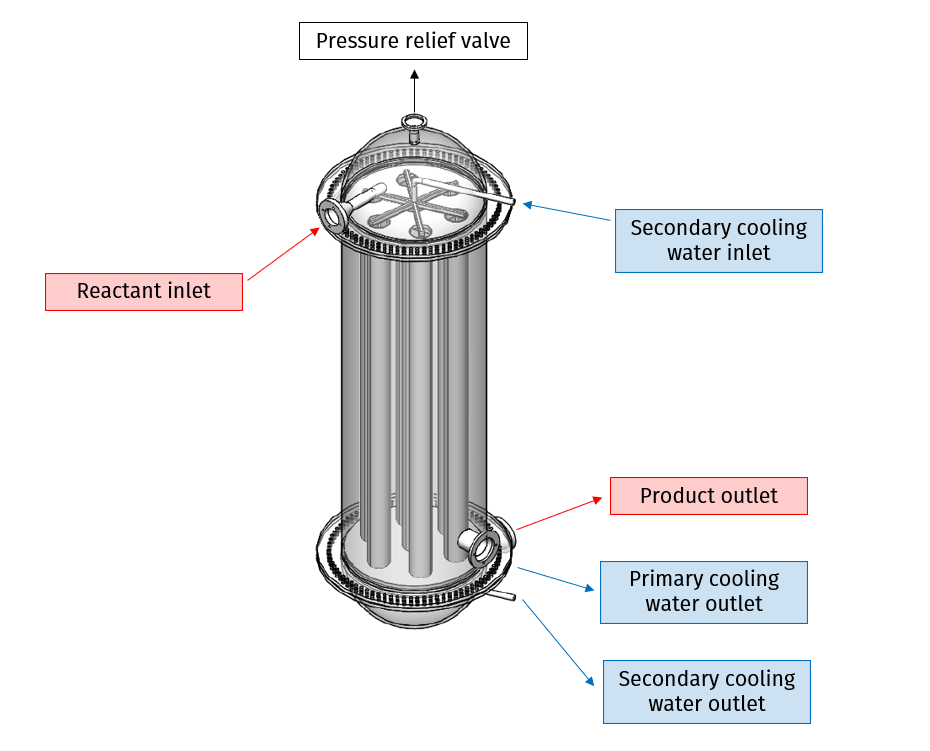
\includegraphics[width=0.8\linewidth]{figures/FYD executive sum.PNG}
        \caption{Mechanical design of nitration reactor}
        \label{fig:executivesummaryreactor}
    \end{minipage}\hfill
    \begin{minipage}[t]{0.45\linewidth}
        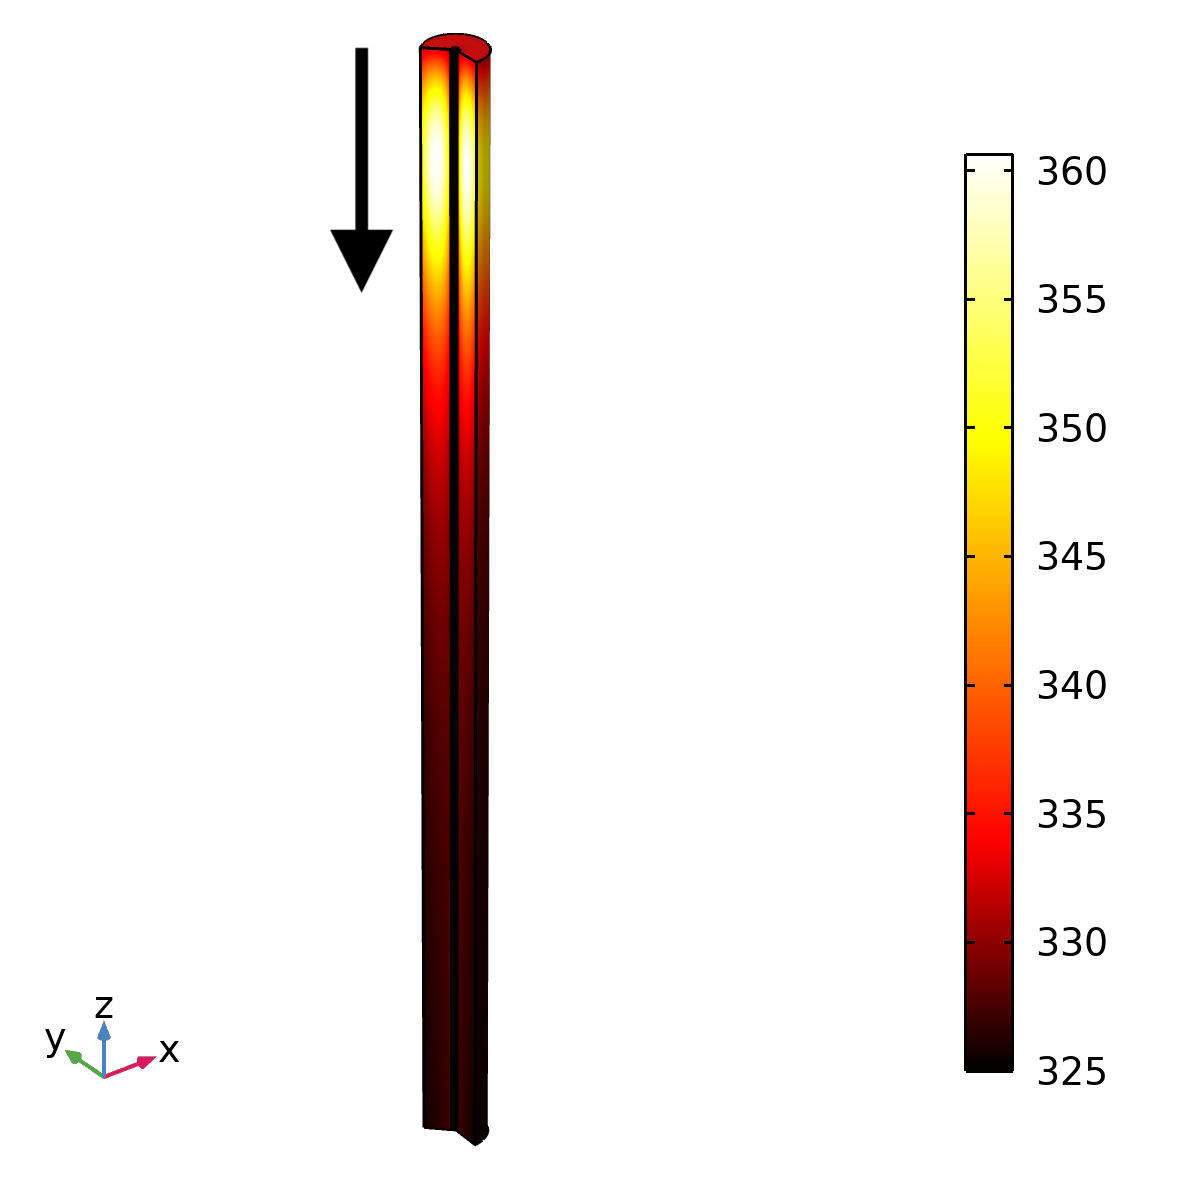
\includegraphics[width=0.8\linewidth]{chapters/2-reaction/figures/temperature-surface-arrow.png}
        \caption{Temperature profile within a reaction tube. Arrow indicates direction of flow.}
        \label{fig:reactor-comsol}
    \end{minipage}
\end{figure}

% The kinetics of the zeolite-catalysed nitration reaction were determined using literature data and the Arrhenius equation. To allow for more accurate modelling, the rate equation for the production of each nitrotoluene isomer was determined. Parameters used in the model were estimated using empirical correlations from literature.

%The reactor is made from stainless steel 304L, which is suitable for corrosive nitric acid processing \cite{cm_selection_nodate}. The wall thickness of the shell and ends were calculated to be 5mm after taking into consideration of corrosion and other welding factors. The final mechanical design can be seen in \cref{fig:executivesummaryreactor}.

Stable reactor operation is also ensured by a detailed mechanical design (\cref{fig:executivesummaryreactor}) that includes using corrosive-resistant stainless steel 304L and sufficient wall thickness \cite{cm_selection_nodate}. Optimal design was achieved after optimisation and sensitivity analyses on the following design parameters: concentric inner cooling pipe diameter and flowrate, direction of cooling water flow, \ch{HNO3} to toluene inlet ratio and total number of reaction tubes. The temperature profile of the reactor, illustrating the performance of the secondary cooling system in reducing hotspot temperature whilst maintaining the required conversion, is shown in \cref{fig:reactor-comsol}. The optimal reactor length was determined to be \SI{4.3}{\m}.  %A further sensitivity analysis was performed on the cooling water inlet temperature since the temperature inside the reactor needs to be well-controlled at all times. Cooling water temperature was simulated to vary by \pm 5 K and the total length of reactor required was investigated. The cooling water is not expected to fluctuate to this degree since it is reused and mixed together from multiple cooling water streams in the plant, but taking a conservative approach to model the reactor increases the overall safety of Nitroma's plant in the worst case scenario. 


